\documentclass[11pt]{article}

\usepackage{graphicx}		% Graphics.
\usepackage{color}
\usepackage[english]{babel}
\usepackage{float}

% Table of Content has fast links to sections.
\usepackage{hyperref}

% Remove dots in table of contents.
\usepackage[titles]{tocloft}
\renewcommand{\cftdot}{}

% Page style.
\usepackage[top=2cm, bottom=2cm, left = 2cm, right = 2cm]{geometry}
\setlength{\parindent}{0pt}	% Disable indents.

\begin{document}

%----------------------------------------------------------------------------------------
%	TITLE PAGE.
%----------------------------------------------------------------------------------------
%----------------------------------------------------------------------------------------
%	TITLE PAGE.
%----------------------------------------------------------------------------------------

\begin{titlepage} % Suppresses displaying the page number on the title page and the subsequent page counts as page 1.
	\center % Centre everything on the page.
	\newcommand{\HRule}{\rule{\linewidth}{0.5mm}} % Defines a new command for horizontal lines, change thickness here.
	
	
	%------------------------------------------------
	%	Logo.
	%------------------------------------------------
	
\includegraphics[width=0.4\textwidth]{figures/LTU_logo.jpg}\\[1cm]
		
	
	%------------------------------------------------
	%	Headings.
	%------------------------------------------------
	\textsc{\Huge Lule\aa \ University of Technology}\\[1.5cm]
	
	\textsc{\LARGE Solar System Project}\\[0.3cm]
	
	\textsc{\large F7008R}\\[0.5cm]
	
	
	%------------------------------------------------
	%	Title.
	%------------------------------------------------
	\HRule\\[0.4cm]
	
	{\Huge\bfseries Are Comets the source of our water?}\\[0.4cm]
	
	\HRule\\[1.5cm]
	
	
	%------------------------------------------------
	%	Author & supervisor.
	%------------------------------------------------
	\begin{minipage}{0.4\textwidth}
		\begin{flushleft}
			\large
			\textit{Authors}\\
			A. Hoehne\\
			A. M\"{o}slinger\\
			E.F.M. Weterings
		\end{flushleft}
	\end{minipage}
	~
	\begin{minipage}{0.4\textwidth}
		\begin{flushright}
			\large
			\textit{Supervisors}\\
			M. Milz\\
			M. Granvik\\
		\end{flushright}
	\end{minipage}
	
	
	%------------------------------------------------
	%	Date.
	%------------------------------------------------
	\vfill\vfill\vfill % Position the date 3/4 down the remaining page.
	
	{\large\today} % Date, change the \today to a set date if you want to be precise.
	
	
\end{titlepage}


%----------------------------------------------------------------------------------------
%	Summary.
%----------------------------------------------------------------------------------------
\newpage				% Start at new page.
\setcounter{page}{0}
\thispagestyle{empty}	% Remove page numbering.
\addcontentsline{toc}{section}{Summary}
%----------------------------------------------------------------------------------------
%	SUMMARY.
%----------------------------------------------------------------------------------------

\section*{Summary}

There are two main theories about the origin of water on Earth: one theory suggests that the inner Solar System was too hot during the creation of planets so no water could aggregate during the formation of the Earth. Therefore, the water must have been brought to Earth after it was formed, presumably by comets and asteroids. While asteroids only contain a maximum relative water amount of approximately 10\%, comets on the other hand mainly consist of water ice (relative water amount usually exceeds 80 or 90\%). During the bombardment of the Earth these objects then have brought particles such as H$_2$O from the depths of the Solar System to Earth. 
The other theory does not exclude the possibility of water particles being brought to Earth with asteroids or comets, however, it claims that the amount of water brought to Earth by extraterrestrial sources by far not enough to fill the oceans, cover the polar caps with ice as well as all the rest of the water that exists on the surface or is stored subterraneously. Therefore, the Earth must have accredited wet.\\

To prove these theories the D/H ratio of water on Earth is compared with the D/H ratio of asteroids and comets. Due to the fact that these objects originate from different parts of the Solar System, their D/H ratios differ, as proven by many measurements on different extraterrestrial bodies as well as the Earth. The results show that the the D/H ratio of an object increases with the distance from the sun of the point of origin. Therefore, the D/H ratio on Earth is smaller than the D/H ratio usually found on comets. However, there are discrepancies in this model as the D/H ratio of Venus is a lot higher than the D/H ratio of the Earth despite the fact that it is closer to the Sun. In addition to this, there are comets such as 103P/Hartley 2 that are believed to originate from the Kuiper belt and have D/H ratios very similar to Earth. These large discrepancies are not yet covered by an updated model. Also, for further research it is essential to measure the D/H ratios of other comets and asteroids to be able to refine these models.\\

As most of the comets have a D/H ratio far higher than that of Earth, the favored theory would be that the Earth accredited wet and only a small fraction of the Earth's water originates from comets and asteroids. Nonetheless, the measurement results from comet 103P/Hartley 2 show very similar results to those on Earth so it is also likely that the Earth accredited dry and gained all its water from comets and asteroids. Before additional research on more asteroids and comets is conducted it is not possible to favor one theory over another.






%----------------------------------------------------------------------------------------
%	TABLE OF CONTENT.
%----------------------------------------------------------------------------------------
\newpage				% Start at new page.
\renewcommand{\contentsname}{Table of Contents}
\tableofcontents		% Add table of content.
\thispagestyle{empty}	% Remove page numbering.


%----------------------------------------------------------------------------------------
%	INTRODUCTION.
%----------------------------------------------------------------------------------------
\newpage				% Start at new page.
\pagenumbering{arabic}	% Page numbering reset & style.
%----------------------------------------------------------------------------------------
%	INTRODUCTION.
%----------------------------------------------------------------------------------------

\section{Introduction}










A simple introduction.\\

D (or HDO) ratio on Earth compared to Comet 67P/Churyumov-Gerasimenko: Are Comets the source of our water?


%----------------------------------------------------------------------------------------
%	CHAPTER: FORMATION COMETS & ASTEROIDS.
%----------------------------------------------------------------------------------------
\newpage
\section{The formation of comets \& asteroids in the early solar system}
How/ where comets/ asteroids/ chondrites/ meteors are created and what this means for the d/h ratio (and perhaps other ratios) of those objects.\\
State how the solar system formed + asteroids and comets (no terestial planets)\\
Anja


%----------------------------------------------------------------------------------------
%	CHAPTER: FORMATION TERRESTRIAL PLANETS.
%----------------------------------------------------------------------------------------
\newpage
%----------------------------------------------------------------------------------------
%	CHAPTER: WATER CONTENT AFTER CREATION TERRESTRIAL PLANETS.
%----------------------------------------------------------------------------------------
\section{Water content of terrestrial planets after their creation}
There is currently no perfect explanation of how the terrestrial planets gained water. The most common hypothesis is that water arrived later on those planets because the temperatures were too high. Therefore the planets accreted dry. This hypothesis is researched in this chapter together with the less famous hypothesis that the planets were accreted wet. For the latter one, also the possibility of holding on to this water is researched.


%----------------------------------------------------------------------------------------
%	PARAGRAPH: FORMATION TERRESTRIAL PLANETS.
%----------------------------------------------------------------------------------------
\subsection{Formation of terrestrial planets in the early solar system}
The terrestrial planets formed from the protoplanetary disk, a large, cold and slowly rotating cloud of gas and dust. The gas and dust sometimes collided due to gravitational forces. If the collisions where gentle enough the gas and dust would grow into a bigger object and eventually into a protoplanet. The gas consisted mostly of hydrogen, helium and oxygen, some of the hydrogen and oxygen combined to make water vapor \cite[p.~523]{TPoriginWater}.\\

The amount of water vapor within 3 AU in the protoplanetary disk has been estimated at three earth masses \cite{TPLecluse} in 1994 and two earth masses \cite{TPPalme} \cite{TPLodders} in 2003. The mass of Earth is $5,9722 \pm 0.0006 \cdot 10^{27}$ g and the earth mass of all Earths oceans is $\pm 1,4 \cdot 10^{24}$ g. The amount of water inside the Earth is not exactly known, most estimations are around 10 Earth oceans with a extreme maximum of 50 Earth oceans \cite[p.~523]{TPoriginWater}. The water storage of Earth in minirals is about 5 - 6 Earth oceans \cite{TPOhtani}.\\

If all four terrestrial planets accreted with 50 Earth oceans of water, then that would still only be 4,7\% of the available water. There was probably enough water vapor in the early solar system to account for Earths oceans and the water on the other terrestrial bodies. The main problem is if the terrestrial bodies could hold on to this water during the formation of the protoplanets due to heat.


%----------------------------------------------------------------------------------------
%	PARAGRAPH: COULD THE TERRESTRIAL PLANETS HOLD ON TO THEIR WATER.
%----------------------------------------------------------------------------------------
\subsection{Water storage in terrestrial planets during formation}
There are two main possibilities of water being stored, hydrated minerals and absorption onto grains. The water can be depleted by high temperatures and collisions. In this paragraph the storage is studied. \\

There are hydrated minerals observed in the mid-asteroid belt. Some were apparently heated to several hundred degrees Celsius. This is a confirmation that water was present at the early solar system and can be stored. The hotter an asteroid would have been, the less of these minerals are found. The chances of the terrestrial bodies holding on to water in hydrated minerals are pretty slim because the temperature of those planets were much higher than those of the asteroids \cite{TPRivkin}.\\

There is also the possibility of water being absorbed by grains. Grains are small objects with a rough surface. The two forms of absorption that could have happened are physisorption and chemisorption \cite[p.~523]{TPoriginWater}. Physisorption is caused by the 'van der Waals force' which is $10 - 100$ meV $\approx 1,6 - 16 \cdot 10^{-21}$ J. Chemisorption involves a chemical reaction between the surface of the grain and in this case water. This force is stronger with $\approx 0,5$ eV $\approx 8 \cdot 10^{-20}$ J.\\

The effects of physisorption has been simulated by creating an Earth out of grains with a 100 times greater surface area than a spherical grain with the same volume. The finding were that with a temperature of 1000 K a quarter of Earths ocean could be absorbed. If the temperature would be 700 K than one Earth ocean would be absorbed and with 500 K three Earth oceans \cite{TPStimpf1} \cite{TPStimpf2}.\\

\newpage
If chemisorption is taken into account the force that keeps the water onto the grains will increase if there are multiple water molecules. How much it exactly contributes is unknown because tests are only performed at temperatures below 30 K. But it can be said that the force that keeps the water onto the grains will increase even at higher temperatures due to chemisorption \cite{TPchemistry}. \\

As the grains collide with each other, some or all of the water will be lost depending on the impact. In the physisorption simulation they accounted for this, if two grains collided with a force greater than two times the total bond energy. In that case all water would be gone. If chemisorption was also taken into consideration the total amount of water that could be stored in the proto-Earth would increase \cite{TPStimpf1} \cite{TPStimpf2}.


%----------------------------------------------------------------------------------------
%	PARAGRAPH: WOULD THE STORED WATER EVAPORRATE AFTER FORMATION.
%----------------------------------------------------------------------------------------
\subsection{Water loss in terrestrial protoplanets}
The early terrestrial planets probably melted one or multiple times while being accreted, probably from multiple major impacts, of which one created the moon. This means that there where magma oceans at some point in their lifetimes, before reaching their final solid state.  \cite{TPformationPlanetesimals}. \\

These magma oceans could have played a key role in delivering volatile into the growing atmosphere through degassing. For this to happen the magma ocean should have been over saturated by these elements and there was no boundary layer for these elements \cite[p.~128-129]{TPmagma}. \\

As the interior gained more heat the volatile elements broke down and formed bubbles that were being transported to the exterior. The melted material would become drier because most volatile elements would migrate to the atmosphere. Most of the big impacts would take away some of the Earths atmosphere but it could also bring other materials to Earth. The impacts would create more heat in the interior and the process of volatile elements out gassing continued until the interior was completely dry \cite[p.~130-131]{TPmagma}.\\

Due to the heat there could not be any oceans on Earth, but the Earth was massive enough to keep most water vapor in the atmosphere. After the Earth cooled down this vapor could condense and become Earths first oceans. Through plate tectonics and volcanic activity more water could be transported from inside the Earth to the oceans \cite[p.~130-131]{TPmagma}.


%----------------------------------------------------------------------------------------
%	PARAGRAPH: D/H RATIOS OF (TERRESTRIAL) PLANETS
%----------------------------------------------------------------------------------------
\newpage
\subsection{The current D/H ratio of terrestrial planets}
The distribution of the D/H ratio through the solar system can be seen in figure \ref{fig:dh-ratio-terrestrial-planets}. It's clear that how further away from the sun, the higher the D/H ratio. Mars has a D/H ratio which is 7 times larger and Venus has a D/H ratio which is 150 times larger. The latter one is a discrepancy because Venus is closer to the sun than Earth. It's possible that Venus got more water from comets from far way in the solar system. This confirms that the origin of water is from comets. Another explanation is that the ultraviolet radiation from the sun breaks water molecules into H and OH, the lighter gass will escape into space. It is possible that Venus lost an ocean’s worth of water but Earth did not because Earth was too far from the Sun for the instability to develop \cite{TPthreeEras}.

\begin{figure}[H]
	\center
	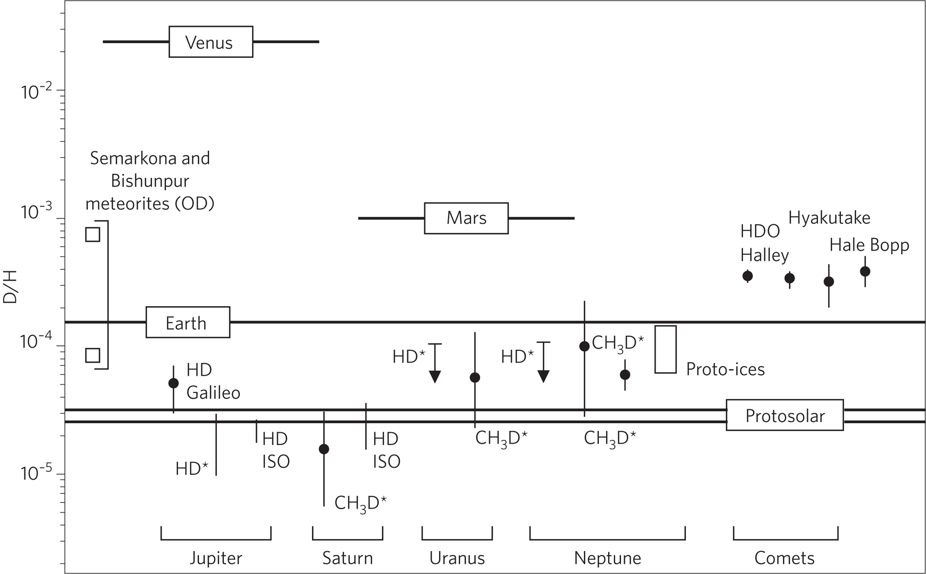
\includegraphics[width=0.75\textwidth]{figures/dh-ratio-terrestrial-planets.jpg}
	\caption{\label{fig:dh-ratio-terrestrial-planets}D/H ratio in the solar system \cite{TPthreeEras}.}
\end{figure}




%----------------------------------------------------------------------------------------
%	CHAPTER: BOMBARDMENT EARTH.
%----------------------------------------------------------------------------------------
\newpage
\section{The bombardment of Earth}
The current amount of water in asteroids is quite low (way lower than comets). Were there enough asteroids to deliver the water to Earth?\\
Wouldn't a comet/asteroid heat up the atmosphere so much that most of the vapor won't get stuck in Earths atmosphere?\\
Where did those asteroids/comets come from?\\
Adam

%----------------------------------------------------------------------------------------
%	CHAPTER: ATMOSPHERE (???DELETE???)
%----------------------------------------------------------------------------------------
\newpage
\section{Earths atmosphere compared to comets \& asteroids}
D/H ratio and atmosphere ratios (like xenon and nitrogen)\\
Probably going to be deleted


%----------------------------------------------------------------------------------------
%	CONCLUSION.
%----------------------------------------------------------------------------------------
\newpage				% Start at new page.
%----------------------------------------------------------------------------------------
%	CONCLUSION & RECOMMENDATIONS.
%----------------------------------------------------------------------------------------

\section{\label{chap:conclusion}Conclusion \& Recommendations}

The era of the origin of Earth has plenty of mysteries and questions remaining to be answered. One of the most important of these questions is about the origin of water on this planet. The answer to this question would reveal how life started to exist and on how other terrestrial planets in other solar systems might develop. This question of the origin of water has been asked and tried to have a satisfactory answer for several decades, no answer has been completely satisfactory. The The main two hypotheses are the Late Heavy Bombardment and the early accretion model. 
The Late Heavy Bombardment says that Earth was formed dry and received water and volatiles from extraplanetary sources. This model dismisses all claims from the early accretion model concerning the possibility of the Earth forming wet. 
The early accretion model does not preclude the Late Heavy Bombardment, however does severely limit the amount of water accumulated from extraplanetary sources. 
The issues with Late Heavy Bombardment is that the isotopes of comets do not match Earth's deuterium to hydrogen ratio; the asteroids have issues with the quantity of hydrated materials. 
The Early Accretion model has issues with retention of water in during the development process.
There is agreement on “our knowledge of detail of terrestrial planet formation and hydration is currently insufficient” \cite{BOMB14}. 

There has been research and modeling that shows only physical absorption or chemical absorption. There should be new research focus on the combination of those two absorption methods to model how much water would be absorbed into grains and minerals. 
The model should determine whether the grains and hydrated minerals would retain water at elevated temperatures that are seen during the development of terrestrial planets.
There should be further research into seeing if the minerals and dust can retain their water at the pressure associated with the impact nature of accretion.
With more research there can be a possible evidence or discrepancy that could make one scenario more or less likely to have occurred.



%----------------------------------------------------------------------------------------
%	RECOMMENDATIONS
%----------------------------------------------------------------------------------------
\newpage				% Start at new page.
%----------------------------------------------------------------------------------------
%	RECOMMENDATIONS.
%----------------------------------------------------------------------------------------

\section{Recommendations}
What can we do/measure to get more information about the origin of water.


%----------------------------------------------------------------------------------------
%	REFERENCES.
%----------------------------------------------------------------------------------------
\newpage				% Start at new page.
\addcontentsline{toc}{section}{References}
\bibliographystyle{ieeetr}
\bibliography{references}


\end{document}